\begin{figure}[H]
    \centering
    


\tikzset{every picture/.style={line width=0.75pt}} %set default line width to 0.75pt        

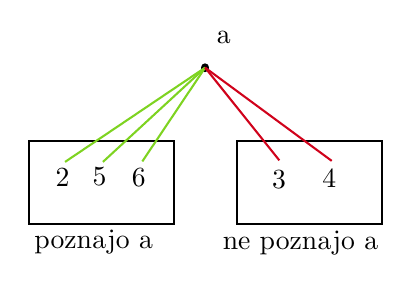
\begin{tikzpicture}[x=0.75pt,y=0.75pt,yscale=-1,xscale=1]
%uncomment if require: \path (0,300); %set diagram left start at 0, and has height of 300

%Shape: Rectangle [id:dp9910313861609417] 
\draw   (80,70.25) -- (150,70.25) -- (150,110.25) -- (80,110.25) -- cycle ;
%Shape: Rectangle [id:dp6524445408103099] 
\draw   (180.25,70) -- (250.25,70) -- (250.25,110) -- (180.25,110) -- cycle ;
%Shape: Free Drawing [id:dp9635620821980186] 
\draw  [line width=3] [line join = round][line cap = round] (165,34.93) .. controls (165,34.84) and (165,34.76) .. (165,34.68) ;
%Straight Lines [id:da8845189038102581] 
\draw [color={rgb, 255:red, 126; green, 211; blue, 33 }  ,draw opacity=1 ]   (165,34.76) -- (97.5,80.18) ;
%Straight Lines [id:da8889347170043365] 
\draw [color={rgb, 255:red, 126; green, 211; blue, 33 }  ,draw opacity=1 ]   (165,34.76) -- (115.75,80.18) ;
%Straight Lines [id:da7198798826573838] 
\draw [color={rgb, 255:red, 126; green, 211; blue, 33 }  ,draw opacity=1 ]   (165,34.76) -- (134.75,79.93) ;
%Straight Lines [id:da7212265299933625] 
\draw [color={rgb, 255:red, 208; green, 2; blue, 27 }  ,draw opacity=1 ]   (165,34.76) -- (200.75,79.43) ;
%Straight Lines [id:da854036126090751] 
\draw [color={rgb, 255:red, 208; green, 2; blue, 27 }  ,draw opacity=1 ]   (165,34.76) -- (226,79.68) ;

% Text Node
\draw (169,16) node [anchor=north west][inner sep=0.75pt]   [align=left] {a};
% Text Node
\draw (91.5,82) node [anchor=north west][inner sep=0.75pt]   [align=left] {2};
% Text Node
\draw (109.25,81.5) node [anchor=north west][inner sep=0.75pt]   [align=left] {5};
% Text Node
\draw (128.25,82) node [anchor=north west][inner sep=0.75pt]   [align=left] {6};
% Text Node
\draw (195.75,82.75) node [anchor=north west][inner sep=0.75pt]   [align=left] {3};
% Text Node
\draw (220,82.5) node [anchor=north west][inner sep=0.75pt]   [align=left] {4};
% Text Node
\draw (81.25,111.5) node [anchor=north west][inner sep=0.75pt]   [align=left] {poznajo a};
% Text Node
\draw (172,111.75) node [anchor=north west][inner sep=0.75pt]   [align=left] {ne poznajo a};


\end{tikzpicture}
\end{figure}